\documentclass{article} % For LaTeX2e
\usepackage{iclr2024_conference,times}

\usepackage[utf8]{inputenc} % allow utf-8 input
\usepackage[T1]{fontenc}    % use 8-bit T1 fonts
\usepackage{hyperref}       % hyperlinks
\usepackage{url}            % simple URL typesetting
\usepackage{booktabs}       % professional-quality tables
\usepackage{amsfonts}       % blackboard math symbols
\usepackage{nicefrac}       % compact symbols for 1/2, etc.
\usepackage{microtype}      % microtypography
\usepackage{titletoc}

\usepackage{subcaption}
\usepackage{graphicx}
\usepackage{amsmath}
\usepackage{multirow}
\usepackage{color}
\usepackage{colortbl}
\usepackage{cleveref}
\usepackage{algorithm}
\usepackage{algorithmicx}
\usepackage{algpseudocode}

\DeclareMathOperator*{\argmin}{arg\,min}
\DeclareMathOperator*{\argmax}{arg\,max}

\graphicspath{{../}} % To reference your generated figures, see below.
\begin{filecontents}{references.bib}

@book{goodfellow2016deep,
  title={Deep learning},
  author={Goodfellow, Ian and Bengio, Yoshua and Courville, Aaron and Bengio, Yoshua},
  volume={1},
  year={2016},
  publisher={MIT Press}
}

@article{vaswani2017attention,
  title={Attention is all you need},
  author={Vaswani, Ashish and Shazeer, Noam and Parmar, Niki and Uszkoreit, Jakob and Jones, Llion and Gomez, Aidan N and Kaiser, {\L}ukasz and Polosukhin, Illia},
  journal={Advances in neural information processing systems},
  volume={30},
  year={2017}
}

@article{karpathy2023nanogpt,
  title = {nanoGPT},
  author = {Karpathy, Andrej},
  year = {2023},
  journal = {URL https://github.com/karpathy/nanoGPT/tree/master},
  note = {GitHub repository}
}

@article{kingma2014adam,
  title={Adam: A method for stochastic optimization},
  author={Kingma, Diederik P and Ba, Jimmy},
  journal={arXiv preprint arXiv:1412.6980},
  year={2014}
}

@article{ba2016layer,
  title={Layer normalization},
  author={Ba, Jimmy Lei and Kiros, Jamie Ryan and Hinton, Geoffrey E},
  journal={arXiv preprint arXiv:1607.06450},
  year={2016}
}

@article{loshchilov2017adamw,
  title={Decoupled weight decay regularization},
  author={Loshchilov, Ilya and Hutter, Frank},
  journal={arXiv preprint arXiv:1711.05101},
  year={2017}
}

@article{radford2019language,
  title={Language Models are Unsupervised Multitask Learners},
  author={Radford, Alec and Wu, Jeff and Child, Rewon and Luan, David and Amodei, Dario and Sutskever, Ilya},
  year={2019}
}

@article{bahdanau2014neural,
  title={Neural machine translation by jointly learning to align and translate},
  author={Bahdanau, Dzmitry and Cho, Kyunghyun and Bengio, Yoshua},
  journal={arXiv preprint arXiv:1409.0473},
  year={2014}
}

@article{paszke2019pytorch,
  title={Pytorch: An imperative style, high-performance deep learning library},
  author={Paszke, Adam and Gross, Sam and Massa, Francisco and Lerer, Adam and Bradbury, James and Chanan, Gregory and Killeen, Trevor and Lin, Zeming and Gimelshein, Natalia and Antiga, Luca and others},
  journal={Advances in neural information processing systems},
  volume={32},
  year={2019}
}

@misc{gpt4,
  title={GPT-4 Technical Report}, 
  author={OpenAI},
  year={2024},
  eprint={2303.08774},
  archivePrefix={arXiv},
  primaryClass={cs.CL},
  url={https://arxiv.org/abs/2303.08774}, 
}

@misc{bussmannBatchTopKSparseAutoencoders2024,
  title = {{{BatchTopK Sparse Autoencoders}}},
  author = {Bussmann, Bart and Leask, Patrick and Nanda, Neel},
  year = {2024},
  month = dec,
  number = {arXiv:2412.06410},
  eprint = {2412.06410},
  primaryclass = {cs},
  publisher = {arXiv},
  doi = {10.48550/arXiv.2412.06410},
  urldate = {2025-01-06},
  abstract = {Sparse autoencoders (SAEs) have emerged as a powerful tool for interpreting language model activations by decomposing them into sparse, interpretable features. A popular approach is the TopK SAE, that uses a fixed number of the most active latents per sample to reconstruct the model activations. We introduce BatchTopK SAEs, a training method that improves upon TopK SAEs by relaxing the topk constraint to the batch-level, allowing for a variable number of latents to be active per sample. As a result, BatchTopK adaptively allocates more or fewer latents depending on the sample, improving reconstruction without sacrificing average sparsity. We show that BatchTopK SAEs consistently outperform TopK SAEs in reconstructing activations from GPT-2 Small and Gemma 2 2B, and achieve comparable performance to state-of-the-art JumpReLU SAEs. However, an advantage of BatchTopK is that the average number of latents can be directly specified, rather than approximately tuned through a costly hyperparameter sweep. We provide code for training and evaluating BatchTopK SAEs at https://github. com/bartbussmann/BatchTopK.},
  archiveprefix = {arXiv},
  langid = {english},
  keywords = {Computer Science - Artificial Intelligence,Computer Science - Machine Learning,Statistics - Machine Learning},
  file = {C:\Users\yanch\Zotero\storage\EJ5UBSNH\Bussmann et al. - 2024 - BatchTopK Sparse Autoencoders.pdf}
}

@misc{chaninAbsorptionStudyingFeature2024,
  title = {A Is for {{Absorption}}: {{Studying Feature Splitting}} and {{Absorption}} in {{Sparse Autoencoders}}},
  shorttitle = {A Is for {{Absorption}}},
  author = {Chanin, David and {Wilken-Smith}, James and Dulka, Tom{\'a}{\v s} and Bhatnagar, Hardik and Bloom, Joseph},
  year = {2024},
  month = sep,
  number = {arXiv:2409.14507},
  eprint = {2409.14507},
  primaryclass = {cs},
  publisher = {arXiv},
  doi = {10.48550/arXiv.2409.14507},
  urldate = {2025-01-27},
  abstract = {Sparse Autoencoders (SAEs) have emerged as a promising approach to decompose the activations of Large Language Models (LLMs) into human-interpretable latents. In this paper, we pose two questions. First, to what extent do SAEs extract monosemantic and interpretable latents? Second, to what extent does varying the sparsity or the size of the SAE affect monosemanticity / interpretability? By investigating these questions in the context of a simple first-letter identification task where we have complete access to ground truth labels for all tokens in the vocabulary, we are able to provide more detail than prior investigations. Critically, we identify a problematic form of feature-splitting we call feature absorption where seemingly monosemantic latents fail to fire in cases where they clearly should. Our investigation suggests that varying SAE size or sparsity is insufficient to solve this issue, and that there are deeper conceptual issues in need of resolution.},
  archiveprefix = {arXiv},
  keywords = {Computer Science - Artificial Intelligence,Computer Science - Computation and Language},
  file = {C\:\\Users\\yanch\\Zotero\\storage\\QIA3MHNG\\Chanin et al. - 2024 - A is for Absorption Studying Feature Splitting an.pdf;C\:\\Users\\yanch\\Zotero\\storage\\FHXMI5CJ\\2409.html}
}

@inproceedings{de-arteagaBiasBiosCase2019,
  title = {Bias in {{Bios}}: {{A Case Study}} of {{Semantic Representation Bias}} in a {{High-Stakes Setting}}},
  shorttitle = {Bias in {{Bios}}},
  booktitle = {Proceedings of the {{Conference}} on {{Fairness}}, {{Accountability}}, and {{Transparency}}},
  author = {{De-Arteaga}, Maria and Romanov, Alexey and Wallach, Hanna and Chayes, Jennifer and Borgs, Christian and Chouldechova, Alexandra and Geyik, Sahin and Kenthapadi, Krishnaram and Kalai, Adam Tauman},
  year = {2019},
  month = jan,
  eprint = {1901.09451},
  primaryclass = {cs},
  pages = {120--128},
  doi = {10.1145/3287560.3287572},
  urldate = {2025-01-27},
  abstract = {We present a large-scale study of gender bias in occupation classification, a task where the use of machine learning may lead to negative outcomes on peoples' lives. We analyze the potential allocation harms that can result from semantic representation bias. To do so, we study the impact on occupation classification of including explicit gender indicators---such as first names and pronouns---in different semantic representations of online biographies. Additionally, we quantify the bias that remains when these indicators are "scrubbed," and describe proxy behavior that occurs in the absence of explicit gender indicators. As we demonstrate, differences in true positive rates between genders are correlated with existing gender imbalances in occupations, which may compound these imbalances.},
  archiveprefix = {arXiv},
  keywords = {Computer Science - Information Retrieval,Computer Science - Machine Learning,Statistics - Machine Learning},
  note = {Comment: Accepted at ACM Conference on Fairness, Accountability, and Transparency (ACM FAT*), 2019},
  file = {C\:\\Users\\yanch\\Zotero\\storage\\SVU9T3AL\\De-Arteaga et al. - 2019 - Bias in Bios A Case Study of Semantic Representat.pdf;C\:\\Users\\yanch\\Zotero\\storage\\MELZABAJ\\1901.html}
}

@misc{farrellApplyingSparseAutoencoders2024,
  title = {Applying Sparse Autoencoders to Unlearn Knowledge in Language Models},
  author = {Farrell, Eoin and Lau, Yeu-Tong and Conmy, Arthur},
  year = {2024},
  month = nov,
  number = {arXiv:2410.19278},
  eprint = {2410.19278},
  primaryclass = {cs},
  publisher = {arXiv},
  doi = {10.48550/arXiv.2410.19278},
  urldate = {2025-01-27},
  abstract = {We investigate whether sparse autoencoders (SAEs) can be used to remove knowledge from language models. We use the biology subset of the Weapons of Mass Destruction Proxy dataset and test on the gemma-2b-it and gemma-2-2b-it language models. We demonstrate that individual interpretable biology-related SAE features can be used to unlearn a subset of WMDP-Bio questions with minimal side-effects in domains other than biology. Our results suggest that negative scaling of feature activations is necessary and that zero ablating features is ineffective. We find that intervening using multiple SAE features simultaneously can unlearn multiple different topics, but with similar or larger unwanted side-effects than the existing Representation Misdirection for Unlearning technique. Current SAE quality or intervention techniques would need to improve to make SAE-based unlearning comparable to the existing fine-tuning based techniques.},
  archiveprefix = {arXiv},
  keywords = {Computer Science - Artificial Intelligence,Computer Science - Machine Learning},
  file = {C\:\\Users\\yanch\\Zotero\\storage\\534ACMZM\\Farrell et al. - 2024 - Applying sparse autoencoders to unlearn knowledge .pdf;C\:\\Users\\yanch\\Zotero\\storage\\2Z3V2URS\\2410.html}
}

@article{gaoScalingEvaluatingSparse,
  title = {Scaling and Evaluating Sparse Autoencoders},
  author = {Gao, Leo and Goh, Gabriel and Sutskever, Ilya},
  langid = {english},
  file = {C:\Users\yanch\Zotero\storage\W35ULTM4\Gao et al. - Scaling and evaluating sparse autoencoders.pdf}
}

@misc{ghilardiEfficientTrainingSparse2024a,
  title = {Efficient {{Training}} of {{Sparse Autoencoders}} for {{Large Language Models}} via {{Layer Groups}}},
  author = {Ghilardi, Davide and Belotti, Federico and Molinari, Marco},
  year = {2024},
  month = oct,
  number = {arXiv:2410.21508},
  eprint = {2410.21508},
  primaryclass = {cs},
  publisher = {arXiv},
  doi = {10.48550/arXiv.2410.21508},
  urldate = {2025-01-06},
  abstract = {Sparse Autoencoders (SAEs) have recently been employed as an unsupervised approach for understanding the inner workings of Large Language Models (LLMs). They reconstruct the model's activations with a sparse linear combination of interpretable features. However, training SAEs is computationally intensive, especially as models grow in size and complexity. To address this challenge, we propose a novel training strategy that reduces the number of trained SAEs from one per layer to one for a given group of contiguous layers. Our experimental results on Pythia 160M highlight a speedup of up to 6x without compromising the reconstruction quality and performance on downstream tasks. Therefore, layer clustering presents an efficient approach to train SAEs in modern LLMs.},
  archiveprefix = {arXiv},
  langid = {english},
  keywords = {Computer Science - Artificial Intelligence,Computer Science - Computation and Language},
  file = {C:\Users\yanch\Zotero\storage\HCBUHHAA\Ghilardi et al. - 2024 - Efficient Training of Sparse Autoencoders for Larg.pdf}
}

@misc{gurneeFindingNeuronsHaystack2023,
  title = {Finding {{Neurons}} in a {{Haystack}}: {{Case Studies}} with {{Sparse Probing}}},
  shorttitle = {Finding {{Neurons}} in a {{Haystack}}},
  author = {Gurnee, Wes and Nanda, Neel and Pauly, Matthew and Harvey, Katherine and Troitskii, Dmitrii and Bertsimas, Dimitris},
  year = {2023},
  month = jun,
  number = {arXiv:2305.01610},
  eprint = {2305.01610},
  primaryclass = {cs},
  publisher = {arXiv},
  doi = {10.48550/arXiv.2305.01610},
  urldate = {2025-01-27},
  abstract = {Despite rapid adoption and deployment of large language models (LLMs), the internal computations of these models remain opaque and poorly understood. In this work, we seek to understand how high-level human-interpretable features are represented within the internal neuron activations of LLMs. We train \$k\$-sparse linear classifiers (probes) on these internal activations to predict the presence of features in the input; by varying the value of \$k\$ we study the sparsity of learned representations and how this varies with model scale. With \$k=1\$, we localize individual neurons which are highly relevant for a particular feature, and perform a number of case studies to illustrate general properties of LLMs. In particular, we show that early layers make use of sparse combinations of neurons to represent many features in superposition, that middle layers have seemingly dedicated neurons to represent higher-level contextual features, and that increasing scale causes representational sparsity to increase on average, but there are multiple types of scaling dynamics. In all, we probe for over 100 unique features comprising 10 different categories in 7 different models spanning 70 million to 6.9 billion parameters.},
  archiveprefix = {arXiv},
  keywords = {Computer Science - Artificial Intelligence,Computer Science - Machine Learning},
  file = {C\:\\Users\\yanch\\Zotero\\storage\\9B43DKLD\\Gurnee et al. - 2023 - Finding Neurons in a Haystack Case Studies with S.pdf;C\:\\Users\\yanch\\Zotero\\storage\\VTA4Y7RU\\2305.html}
}

@misc{InterpretabilityCompressionReconsidering,
  title = {Interpretability as {{Compression}}: {{Reconsidering SAE Explanations}} of {{Neural Activations}} with {{MDL-SAEs}}},
  urldate = {2025-01-15},
  howpublished = {https://arxiv.org/html/2410.11179v1},
  file = {C:\Users\yanch\Zotero\storage\S3LK2LEB\2410.html}
}

@misc{karvonenEvaluatingSparseAutoencoders2024,
  title = {Evaluating {{Sparse Autoencoders}} on {{Targeted Concept Erasure Tasks}}},
  author = {Karvonen, Adam and Rager, Can and Marks, Samuel and Nanda, Neel},
  year = {2024},
  month = nov,
  number = {arXiv:2411.18895},
  eprint = {2411.18895},
  primaryclass = {cs},
  publisher = {arXiv},
  doi = {10.48550/arXiv.2411.18895},
  urldate = {2025-01-27},
  abstract = {Sparse Autoencoders (SAEs) are an interpretability technique aimed at decomposing neural network activations into interpretable units. However, a major bottleneck for SAE development has been the lack of high-quality performance metrics, with prior work largely relying on unsupervised proxies. In this work, we introduce a family of evaluations based on SHIFT, a downstream task from Marks et al. (Sparse Feature Circuits, 2024) in which spurious cues are removed from a classifier by ablating SAE features judged to be task-irrelevant by a human annotator. We adapt SHIFT into an automated metric of SAE quality; this involves replacing the human annotator with an LLM. Additionally, we introduce the Targeted Probe Perturbation (TPP) metric that quantifies an SAE's ability to disentangle similar concepts, effectively scaling SHIFT to a wider range of datasets. We apply both SHIFT and TPP to multiple open-source models, demonstrating that these metrics effectively differentiate between various SAE training hyperparameters and architectures.},
  archiveprefix = {arXiv},
  keywords = {Computer Science - Computation and Language,Computer Science - Machine Learning},
  file = {C\:\\Users\\yanch\\Zotero\\storage\\HRKJ9X7I\\Karvonen et al. - 2024 - Evaluating Sparse Autoencoders on Targeted Concept.pdf;C\:\\Users\\yanch\\Zotero\\storage\\7P5P4TUP\\2411.html}
}

@misc{liWMDPBenchmarkMeasuring2024,
  title = {The {{WMDP Benchmark}}: {{Measuring}} and {{Reducing Malicious Use With Unlearning}}},
  shorttitle = {The {{WMDP Benchmark}}},
  author = {Li, Nathaniel and Pan, Alexander and Gopal, Anjali and Yue, Summer and Berrios, Daniel and Gatti, Alice and Li, Justin D. and Dombrowski, Ann-Kathrin and Goel, Shashwat and Phan, Long and Mukobi, Gabriel and {Helm-Burger}, Nathan and Lababidi, Rassin and Justen, Lennart and Liu, Andrew B. and Chen, Michael and Barrass, Isabelle and Zhang, Oliver and Zhu, Xiaoyuan and Tamirisa, Rishub and Bharathi, Bhrugu and Khoja, Adam and Zhao, Zhenqi and {Herbert-Voss}, Ariel and Breuer, Cort B. and Marks, Samuel and Patel, Oam and Zou, Andy and Mazeika, Mantas and Wang, Zifan and Oswal, Palash and Lin, Weiran and Hunt, Adam A. and {Tienken-Harder}, Justin and Shih, Kevin Y. and Talley, Kemper and Guan, John and Kaplan, Russell and Steneker, Ian and Campbell, David and Jokubaitis, Brad and Levinson, Alex and Wang, Jean and Qian, William and Karmakar, Kallol Krishna and Basart, Steven and Fitz, Stephen and Levine, Mindy and Kumaraguru, Ponnurangam and Tupakula, Uday and Varadharajan, Vijay and Wang, Ruoyu and Shoshitaishvili, Yan and Ba, Jimmy and Esvelt, Kevin M. and Wang, Alexandr and Hendrycks, Dan},
  year = {2024},
  month = may,
  number = {arXiv:2403.03218},
  eprint = {2403.03218},
  primaryclass = {cs},
  publisher = {arXiv},
  doi = {10.48550/arXiv.2403.03218},
  urldate = {2025-01-27},
  abstract = {The White House Executive Order on Artificial Intelligence highlights the risks of large language models (LLMs) empowering malicious actors in developing biological, cyber, and chemical weapons. To measure these risks of malicious use, government institutions and major AI labs are developing evaluations for hazardous capabilities in LLMs. However, current evaluations are private, preventing further research into mitigating risk. Furthermore, they focus on only a few, highly specific pathways for malicious use. To fill these gaps, we publicly release the Weapons of Mass Destruction Proxy (WMDP) benchmark, a dataset of 3,668 multiple-choice questions that serve as a proxy measurement of hazardous knowledge in biosecurity, cybersecurity, and chemical security. WMDP was developed by a consortium of academics and technical consultants, and was stringently filtered to eliminate sensitive information prior to public release. WMDP serves two roles: first, as an evaluation for hazardous knowledge in LLMs, and second, as a benchmark for unlearning methods to remove such hazardous knowledge. To guide progress on unlearning, we develop RMU, a state-of-the-art unlearning method based on controlling model representations. RMU reduces model performance on WMDP while maintaining general capabilities in areas such as biology and computer science, suggesting that unlearning may be a concrete path towards reducing malicious use from LLMs. We release our benchmark and code publicly at https://wmdp.ai},
  archiveprefix = {arXiv},
  keywords = {Computer Science - Artificial Intelligence,Computer Science - Computation and Language,Computer Science - Computers and Society,Computer Science - Machine Learning},
  note = {Comment: See the project page at https://wmdp.ai},
  file = {C\:\\Users\\yanch\\Zotero\\storage\\IH8WJB8J\\Li et al. - 2024 - The WMDP Benchmark Measuring and Reducing Malicio.pdf;C\:\\Users\\yanch\\Zotero\\storage\\PI5CUBZH\\2403.html}
}

@misc{marksSparseFeatureCircuits2024,
  title = {Sparse {{Feature Circuits}}: {{Discovering}} and {{Editing Interpretable Causal Graphs}} in {{Language Models}}},
  shorttitle = {Sparse {{Feature Circuits}}},
  author = {Marks, Samuel and Rager, Can and Michaud, Eric J. and Belinkov, Yonatan and Bau, David and Mueller, Aaron},
  year = {2024},
  month = mar,
  number = {arXiv:2403.19647},
  eprint = {2403.19647},
  primaryclass = {cs},
  publisher = {arXiv},
  doi = {10.48550/arXiv.2403.19647},
  urldate = {2025-01-27},
  abstract = {We introduce methods for discovering and applying sparse feature circuits. These are causally implicated subnetworks of human-interpretable features for explaining language model behaviors. Circuits identified in prior work consist of polysemantic and difficult-to-interpret units like attention heads or neurons, rendering them unsuitable for many downstream applications. In contrast, sparse feature circuits enable detailed understanding of unanticipated mechanisms. Because they are based on fine-grained units, sparse feature circuits are useful for downstream tasks: We introduce SHIFT, where we improve the generalization of a classifier by ablating features that a human judges to be task-irrelevant. Finally, we demonstrate an entirely unsupervised and scalable interpretability pipeline by discovering thousands of sparse feature circuits for automatically discovered model behaviors.},
  archiveprefix = {arXiv},
  keywords = {Computer Science - Artificial Intelligence,Computer Science - Computation and Language,Computer Science - Machine Learning},
  note = {Comment: Code and data at https://github.com/saprmarks/feature-circuits. Demonstration at https://feature-circuits.xyz},
  file = {C\:\\Users\\yanch\\Zotero\\storage\\U9MWC7I4\\Marks et al. - 2024 - Sparse Feature Circuits Discovering and Editing I.pdf;C\:\\Users\\yanch\\Zotero\\storage\\AML7HRZK\\2403.html}
}

@misc{mudideEfficientDictionaryLearning2024a,
  title = {Efficient {{Dictionary Learning}} with {{Switch Sparse Autoencoders}}},
  author = {Mudide, Anish and Engels, Joshua and Michaud, Eric J. and Tegmark, Max and de Witt, Christian Schroeder},
  year = {2024},
  month = oct,
  number = {arXiv:2410.08201},
  eprint = {2410.08201},
  primaryclass = {cs},
  publisher = {arXiv},
  doi = {10.48550/arXiv.2410.08201},
  urldate = {2025-01-06},
  abstract = {Sparse autoencoders (SAEs) are a recent technique for decomposing neural network activations into human-interpretable features. However, in order for SAEs to identify all features represented in frontier models, it will be necessary to scale them up to very high width, posing a computational challenge. In this work, we introduce Switch Sparse Autoencoders, a novel SAE architecture aimed at reducing the compute cost of training SAEs. Inspired by sparse mixture of experts models, Switch SAEs route activation vectors between smaller ``expert'' SAEs, enabling SAEs to efficiently scale to many more features. We present experiments comparing Switch SAEs with other SAE architectures, and find that Switch SAEs deliver a substantial Pareto improvement in the reconstruction vs. sparsity frontier for a given fixed training compute budget. We also study the geometry of features across experts, analyze features duplicated across experts, and verify that Switch SAE features are as interpretable as features found by other SAE architectures.},
  archiveprefix = {arXiv},
  langid = {english},
  keywords = {Computer Science - Machine Learning},
  note = {Comment: Code available at https://github.com/amudide/switch\_sae},
  file = {C:\Users\yanch\Zotero\storage\ZZUFEFUK\Mudide et al. - 2024 - Efficient Dictionary Learning with Switch Sparse A.pdf}
}

@misc{pauloAutomaticallyInterpretingMillions2024,
  title = {Automatically {{Interpreting Millions}} of {{Features}} in {{Large Language Models}}},
  author = {Paulo, Gon{\c c}alo and Mallen, Alex and Juang, Caden and Belrose, Nora},
  year = {2024},
  month = dec,
  number = {arXiv:2410.13928},
  eprint = {2410.13928},
  primaryclass = {cs},
  publisher = {arXiv},
  doi = {10.48550/arXiv.2410.13928},
  urldate = {2025-01-27},
  abstract = {While the activations of neurons in deep neural networks usually do not have a simple human-understandable interpretation, sparse autoencoders (SAEs) can be used to transform these activations into a higher-dimensional latent space which may be more easily interpretable. However, these SAEs can have millions of distinct latent features, making it infeasible for humans to manually interpret each one. In this work, we build an open-source automated pipeline to generate and evaluate natural language explanations for SAE features using LLMs. We test our framework on SAEs of varying sizes, activation functions, and losses, trained on two different open-weight LLMs. We introduce five new techniques to score the quality of explanations that are cheaper to run than the previous state of the art. One of these techniques, intervention scoring, evaluates the interpretability of the effects of intervening on a feature, which we find explains features that are not recalled by existing methods. We propose guidelines for generating better explanations that remain valid for a broader set of activating contexts, and discuss pitfalls with existing scoring techniques. We use our explanations to measure the semantic similarity of independently trained SAEs, and find that SAEs trained on nearby layers of the residual stream are highly similar. Our large-scale analysis confirms that SAE latents are indeed much more interpretable than neurons, even when neurons are sparsified using top-\$k\$ postprocessing. Our code is available at https://github.com/EleutherAI/sae-auto-interp, and our explanations are available at https://huggingface.co/datasets/EleutherAI/auto\_interp\_explanations.},
  archiveprefix = {arXiv},
  keywords = {Computer Science - Computation and Language,Computer Science - Machine Learning},
  file = {C\:\\Users\\yanch\\Zotero\\storage\\7ADXVWT6\\Paulo et al. - 2024 - Automatically Interpreting Millions of Features in.pdf;C\:\\Users\\yanch\\Zotero\\storage\\5HVTWCYX\\2410.html}
}

@misc{rajamanoharanImprovingDictionaryLearning2024,
  title = {Improving {{Dictionary Learning}} with {{Gated Sparse Autoencoders}}},
  author = {Rajamanoharan, Senthooran and Conmy, Arthur and Smith, Lewis and Lieberum, Tom and Varma, Vikrant and Kram{\'a}r, J{\'a}nos and Shah, Rohin and Nanda, Neel},
  year = {2024},
  month = apr,
  number = {arXiv:2404.16014},
  eprint = {2404.16014},
  primaryclass = {cs},
  publisher = {arXiv},
  doi = {10.48550/arXiv.2404.16014},
  urldate = {2025-01-06},
  abstract = {Recent work has found that sparse autoencoders (SAEs) are an effective technique for unsupervised discovery of interpretable features in language models' (LMs) activations, by finding sparse, linear reconstructions of LM activations. We introduce the Gated Sparse Autoencoder (Gated SAE), which achieves a Pareto improvement over training with prevailing methods. In SAEs, the L1 penalty used to encourage sparsity introduces many undesirable biases, such as shrinkage -- systematic underestimation of feature activations. The key insight of Gated SAEs is to separate the functionality of (a) determining which directions to use and (b) estimating the magnitudes of those directions: this enables us to apply the L1 penalty only to the former, limiting the scope of undesirable side effects. Through training SAEs on LMs of up to 7B parameters we find that, in typical hyper-parameter ranges, Gated SAEs solve shrinkage, are similarly interpretable, and require half as many firing features to achieve comparable reconstruction fidelity.},
  archiveprefix = {arXiv},
  langid = {english},
  keywords = {Computer Science - Artificial Intelligence,Computer Science - Machine Learning},
  note = {Comment: 15 main text pages, 22 appendix pages},
  file = {C:\Users\yanch\Zotero\storage\FWEYSUFQ\Rajamanoharan et al. - 2024 - Improving Dictionary Learning with Gated Sparse Au.pdf}
}

@misc{rajamanoharanJumpingAheadImproving2024,
  title = {Jumping {{Ahead}}: {{Improving Reconstruction Fidelity}} with {{JumpReLU Sparse Autoencoders}}},
  shorttitle = {Jumping {{Ahead}}},
  author = {Rajamanoharan, Senthooran and Lieberum, Tom and Sonnerat, Nicolas and Conmy, Arthur and Varma, Vikrant and Kram{\'a}r, J{\'a}nos and Nanda, Neel},
  year = {2024},
  month = aug,
  number = {arXiv:2407.14435},
  eprint = {2407.14435},
  primaryclass = {cs},
  publisher = {arXiv},
  doi = {10.48550/arXiv.2407.14435},
  urldate = {2025-01-06},
  abstract = {Sparse autoencoders (SAEs) are a promising unsupervised approach for identifying causally relevant and interpretable linear features in a language model's (LM) activations. To be useful for downstream tasks, SAEs need to decompose LM activations faithfully; yet to be interpretable the decomposition must be sparse -- two objectives that are in tension. In this paper, we introduce JumpReLU SAEs, which achieve state-of-the-art reconstruction fidelity at a given sparsity level on Gemma 2 9B activations, compared to other recent advances such as Gated and TopK SAEs. We also show that this improvement does not come at the cost of interpretability through manual and automated interpretability studies. JumpReLU SAEs are a simple modification of vanilla (ReLU) SAEs -- where we replace the ReLU with a discontinuous JumpReLU activation function -- and are similarly efficient to train and run. By utilising straight-through-estimators (STEs) in a principled manner, we show how it is possible to train JumpReLU SAEs effectively despite the discontinuous JumpReLU function introduced in the SAE's forward pass. Similarly, we use STEs to directly train L0 to be sparse, instead of training on proxies such as L1, avoiding problems like shrinkage.},
  archiveprefix = {arXiv},
  langid = {english},
  keywords = {Computer Science - Machine Learning},
  note = {Comment: v2: new appendix H comparing kernel functions \& bug-fixes to pseudo-code in Appendix J v3: further bug-fix to pseudo-code in Appendix J},
  file = {C:\Users\yanch\Zotero\storage\Q7MG9Z77\Rajamanoharan et al. - 2024 - Jumping Ahead Improving Reconstruction Fidelity w.pdf}
}

@article{hou2024bridging,
  title={Bridging Language and Items for Retrieval and Recommendation},
  author={Hou, Yupeng and Li, Jiacheng and He, Zhankui and Yan, An and Chen, Xiusi and McAuley, Julian},
  journal={arXiv preprint arXiv:2403.03952},
  year={2024}
}


@Article{Olshausen1996EmergenceOS,
 author = {B. Olshausen and D. Field},
 booktitle = {Nature},
 journal = {Nature},
 pages = {607-609},
 title = {Emergence of simple-cell receptive field properties by learning a sparse code for natural images},
 volume = {381},
 year = {1996}
}


@Article{Hoyer2002NonnegativeSC,
 author = {P. Hoyer},
 booktitle = {Proceedings of the 12th IEEE Workshop on Neural Networks for Signal Processing},
 journal = {Proceedings of the 12th IEEE Workshop on Neural Networks for Signal Processing},
 pages = {557-565},
 title = {Non-negative sparse coding},
 year = {2002}
}


@Article{Bell1995AnIA,
 author = {A. J. Bell and T. Sejnowski},
 booktitle = {Neural Computation},
 journal = {Neural Computation},
 pages = {1129-1159},
 title = {An Information-Maximization Approach to Blind Separation and Blind Deconvolution},
 volume = {7},
 year = {1995}
}


@Article{Olshausen1996EmergenceOS,
 author = {B. Olshausen and D. Field},
 booktitle = {Nature},
 journal = {Nature},
 pages = {607-609},
 title = {Emergence of simple-cell receptive field properties by learning a sparse code for natural images},
 volume = {381},
 year = {1996}
}


@Article{Lee1999LearningTP,
 author = {Daniel D. Lee and H. S. Seung},
 booktitle = {Nature},
 journal = {Nature},
 pages = {788-791},
 title = {Learning the parts of objects by non-negative matrix factorization},
 volume = {401},
 year = {1999}
}


@Article{Hyvärinen2000IndependentCA,
 author = {Aapo Hyvärinen and E. Oja},
 booktitle = {Neural Networks},
 journal = {Neural networks : the official journal of the International Neural Network Society},
 pages = {
          411-30
        },
 title = {Independent component analysis: algorithms and applications},
 volume = {13 4-5},
 year = {2000}
}


@Article{Olshausen1996EmergenceOS,
 author = {B. Olshausen and D. Field},
 booktitle = {Nature},
 journal = {Nature},
 pages = {607-609},
 title = {Emergence of simple-cell receptive field properties by learning a sparse code for natural images},
 volume = {381},
 year = {1996}
}


@Article{Bengio2007LearningDA,
 author = {Yoshua Bengio},
 booktitle = {Found. Trends Mach. Learn.},
 journal = {Found. Trends Mach. Learn.},
 pages = {1-127},
 title = {Learning Deep Architectures for AI},
 volume = {2},
 year = {2007}
}


@Article{He2015DeepRL,
 author = {Kaiming He and X. Zhang and Shaoqing Ren and Jian Sun},
 booktitle = {Computer Vision and Pattern Recognition},
 journal = {2016 IEEE Conference on Computer Vision and Pattern Recognition (CVPR)},
 pages = {770-778},
 title = {Deep Residual Learning for Image Recognition},
 year = {2015}
}


@Article{He2015DeepRL,
 author = {Kaiming He and X. Zhang and Shaoqing Ren and Jian Sun},
 booktitle = {Computer Vision and Pattern Recognition},
 journal = {2016 IEEE Conference on Computer Vision and Pattern Recognition (CVPR)},
 pages = {770-778},
 title = {Deep Residual Learning for Image Recognition},
 year = {2015}
}


@Article{Cunningham2023SparseAF,
 author = {Hoagy Cunningham and Aidan Ewart and Logan Riggs and R. Huben and Lee Sharkey},
 booktitle = {International Conference on Learning Representations},
 journal = {ArXiv},
 title = {Sparse Autoencoders Find Highly Interpretable Features in Language Models},
 volume = {abs/2309.08600},
 year = {2023}
}


@Article{Olshausen1996EmergenceOS,
 author = {B. Olshausen and D. Field},
 booktitle = {Nature},
 journal = {Nature},
 pages = {607-609},
 title = {Emergence of simple-cell receptive field properties by learning a sparse code for natural images},
 volume = {381},
 year = {1996}
}


@Article{Hoyer2002NonnegativeSC,
 author = {P. Hoyer},
 booktitle = {Proceedings of the 12th IEEE Workshop on Neural Networks for Signal Processing},
 journal = {Proceedings of the 12th IEEE Workshop on Neural Networks for Signal Processing},
 pages = {557-565},
 title = {Non-negative sparse coding},
 year = {2002}
}


@Article{Olshausen1996EmergenceOS,
 author = {B. Olshausen and D. Field},
 booktitle = {Nature},
 journal = {Nature},
 pages = {607-609},
 title = {Emergence of simple-cell receptive field properties by learning a sparse code for natural images},
 volume = {381},
 year = {1996}
}


@Article{Olshausen1996EmergenceOS,
 author = {B. Olshausen and D. Field},
 booktitle = {Nature},
 journal = {Nature},
 pages = {607-609},
 title = {Emergence of simple-cell receptive field properties by learning a sparse code for natural images},
 volume = {381},
 year = {1996}
}


@Article{Ranzato2007SparseFL,
 author = {Marc'Aurelio Ranzato and Y-Lan Boureau and Yann LeCun},
 booktitle = {Neural Information Processing Systems},
 pages = {1185-1192},
 title = {Sparse Feature Learning for Deep Belief Networks},
 year = {2007}
}

\end{filecontents}

\title{Ordered Minds: Frequency-Based Feature Organization for Interpretable Neural Representations}

\author{LLM\\
Department of Computer Science\\
University of LLMs\\
}

\newcommand{\fix}{\marginpar{FIX}}
\newcommand{\new}{\marginpar{NEW}}

\begin{document}

\maketitle

\begin{abstract}
Understanding the internal representations of large language models is crucial for ensuring their safe and reliable deployment, yet current interpretability methods struggle to organize learned features in a systematic way. We present Frequency-Ordered Sparse Autoencoders (FOSAEs), which address this challenge by introducing a frequency-based ordering constraint that structures learned features according to their activation patterns. This ordering enables more efficient analysis by placing frequently activated features earlier in the feature sequence, creating a natural hierarchy for investigation. Through experiments on the Gemma-2-2B language model, we demonstrate that FOSAEs achieve exceptional performance while maintaining interpretability: our architecture combines state-of-the-art reconstruction quality (0.969 cosine similarity) with strong model behavior preservation (0.990 KL divergence) and high sparsity (L0 norm 23.82). The effectiveness of our frequency-based ordering is validated through absorption studies showing balanced feature distribution across 22 letter-specific concepts, with consistent interpretability scores (mean 0.010) maintained throughout training. By combining adaptive penalties, layer normalization, skip connections, and self-attention mechanisms, FOSAEs advance our ability to systematically analyze and understand large language models.
\end{abstract}

\section{Introduction}
\label{sec:intro}

Understanding the internal representations of large language models (LLMs) has become increasingly crucial as these models are deployed in high-stakes applications \cite{de-arteagaBiasBiosCase2019}. While sparse autoencoders (SAEs) have emerged as a promising approach for decomposing neural activations into interpretable features \cite{gaoScalingEvaluatingSparse}, current methods face two critical challenges: (1) learned features lack systematic organization, making analysis of thousands of features unnecessarily complex, and (2) existing architectures struggle to balance reconstruction quality with interpretability \cite{rajamanoharanJumpingAheadImproving2024}.

We present Frequency-Ordered Sparse Autoencoders (FOSAEs), which address these challenges by introducing a frequency-based ordering constraint that structures learned features according to their activation patterns. This ordering enables more efficient analysis by placing frequently activated features earlier in the feature sequence, creating a natural hierarchy for investigation. Our approach builds upon recent advances in SAE architecture \cite{rajamanoharanImprovingDictionaryLearning2024}, incorporating adaptive penalties, normalization, and attention mechanisms to achieve state-of-the-art performance while maintaining interpretability.

Our key technical contributions include:
\begin{itemize}
    \item A novel frequency-based ordering mechanism that creates interpretable feature hierarchies while maintaining strong reconstruction quality (0.969 cosine similarity)
    \item An adaptive L1 penalty scheme that achieves high sparsity (L0 norm 23.82) while preserving model behavior (0.990 KL divergence)
    \item A comprehensive architecture combining layer normalization, skip connections, and self-attention mechanisms, validated through extensive ablation studies
    \item A robust feature resampling strategy ensuring balanced feature utilization, demonstrated by consistent absorption scores (mean 0.010) across 22 letter-specific concepts
\end{itemize}

Through systematic experiments on the Gemma-2-2B language model, we demonstrate FOSAEs' effectiveness across multiple evaluation dimensions. Our nine architectural iterations, documented with detailed ablation studies, show how each component contributes to the final performance. The frequency ordering mechanism creates clear feature hierarchies while maintaining strong reconstruction quality and interpretability metrics. Notably, our approach achieves these results without sacrificing computational efficiency, requiring only modest additional overhead for frequency tracking.

Looking ahead, FOSAEs open new possibilities for structured model interpretation. The ordered feature representations enable more systematic analysis of model behavior, particularly valuable for ongoing work in model safety \cite{liWMDPBenchmarkMeasuring2024} and targeted concept manipulation \cite{farrell2024applying}. Future work could explore dynamic ordering schemes, applications to larger models, and integration with complementary interpretability techniques.


\section{Related Work}
\label{sec:related}
Our work builds on recent advances in sparse autoencoder design while addressing the critical challenge of systematic feature organization. Three main approaches have emerged for improving SAE interpretability:

First, architectural innovations have focused on activation functions and feature selection. JumpReLU SAEs \cite{rajamanoharanJumpingAheadImproving2024} achieve strong reconstruction (0.95 cosine similarity) using discontinuous activations, but their binary nature makes ordering features challenging. Our continuous activation approach enables smoother frequency-based organization while achieving comparable reconstruction (0.969). Gated SAEs \cite{rajamanoharanImprovingDictionaryLearning2024} reduce shrinkage bias by separating feature selection from magnitude estimation, a principle we incorporate through our adaptive L1 penalty while adding frequency ordering.

Second, approaches to feature organization have explored different granularities. Switch SAEs \cite{mudideEfficientDictionaryLearning2024a} distribute features across expert networks for computational efficiency but sacrifice global feature relationships. Our single-network approach maintains these relationships while achieving comparable efficiency through frequency-based pruning. Layer Groups \cite{ghilardiEfficientTrainingSparse2024a} organize features hierarchically across model layers, showing 6x speedup but potentially missing within-layer patterns. Our within-layer ordering complements their approach and could be integrated for multi-level organization.

Third, evaluation methods have become increasingly sophisticated. While absorption studies \cite{chaninAbsorptionStudyingFeature2024} focus on feature monosemanticity and sparse probing \cite{gurneeFindingNeuronsHaystack2023} examines localization, neither addresses the systematic organization of features. Our frequency-based metrics provide a new dimension for evaluation while maintaining strong performance on existing metrics (0.010 absorption score, balanced across 22/26 letters). This enables quantitative comparison of feature organization strategies, a capability missing from previous frameworks.

\section{Background}
\label{sec:background}

Sparse coding has a rich history in computational neuroscience and machine learning, originating from studies of visual cortex organization \cite{Olshausen1996EmergenceOS}. This work demonstrated that sparse, overcomplete representations naturally emerge when optimizing for both reconstruction accuracy and activation sparsity. These principles were further developed through non-negative sparse coding \cite{Hoyer2002NonnegativeSC} and independent component analysis \cite{Bell1995AnIA}, establishing the theoretical foundations for modern sparse autoencoders.

The transition to deep learning brought new challenges and opportunities \cite{Bengio2007LearningDA}, particularly in handling the increased complexity of learned representations. Recent work applying sparse autoencoders to language models \cite{Cunningham2023SparseAF} has shown promising results in decomposing neural activations into interpretable features, though the challenge of organizing these features remains largely unaddressed.

\subsection{Problem Setting}
Given a pre-trained language model $M$ with hidden dimension $d$, we observe activations $h \in \mathbb{R}^d$ at a specific layer $l$. Our goal is to learn an encoder $E: \mathbb{R}^d \to \mathbb{R}^k$ and decoder $D: \mathbb{R}^k \to \mathbb{R}^d$ where $k > d$ (overcomplete representation), such that:

1. The reconstruction $D(E(h))$ accurately preserves the original activations $h$
2. The encoded features $z = E(h)$ are sparse (few non-zero elements)
3. Features are ordered by activation frequency: $f_i \geq f_{i+1}$ for all $i$

where $f_i = \mathbb{E}_{h \sim \mathcal{D}}[\mathbbm{1}(|z_i| > \epsilon)]$ is the activation frequency of feature $i$.

Key assumptions in our approach:
\begin{itemize}
    \item Feature interpretability correlates with activation sparsity
    \item More frequently activated features carry greater importance for model behavior
    \item The distribution of feature frequencies follows a natural ordering
\end{itemize}

These assumptions are validated through our experimental results, particularly the absorption studies showing consistent interpretability scores across training iterations.

\section{Method}
\label{sec:method}

Building on the sparse coding foundations introduced in Section \ref{sec:background}, we present Frequency-Ordered Sparse Autoencoders (FOSAEs). Our key insight is that organizing features by activation frequency creates an interpretable hierarchy while maintaining the benefits of sparse representations established by \cite{Olshausen1996EmergenceOS}.

\subsection{Architecture}
Given input activations $h \in \mathbb{R}^d$, our encoder $E$ and decoder $D$ are defined as:

\begin{align}
z &= \text{ReLU}(\text{LayerNorm}(W_E h + b_E) + \alpha \text{Skip}(h)) \\
\hat{h} &= W_D z + b_D
\end{align}

where $W_E \in \mathbb{R}^{k \times d}$, $W_D \in \mathbb{R}^{d \times k}$ are the encoding and decoding matrices, $b_E \in \mathbb{R}^k$, $b_D \in \mathbb{R}^d$ are bias terms, and $\alpha=0.1$ controls the skip connection strength. The skip projection $\text{Skip}(h) = W_S h$ helps maintain gradient flow during training.

\subsection{Frequency-Based Ordering}
We track feature activation frequencies $f_i$ across training batches:

\begin{equation}
f_i = \frac{1}{T} \sum_{t=1}^T \mathbb{E}_{h \sim \mathcal{B}_t}[\mathbbm{1}(|z_i| > \epsilon)]
\end{equation}

where $T$ is the number of batches and $\epsilon=10^{-4}$ is the activation threshold. The ordering constraint is enforced through:

\begin{equation}
\mathcal{L}_{\text{order}} = \lambda_2 \sum_{i=1}^{k-1} \text{ReLU}(f_{i+1} - f_i)
\end{equation}

where $\lambda_2=0.3$ controls the strength of the ordering penalty.

\subsection{Training Objectives}
The total loss combines reconstruction, sparsity, and ordering terms:

\begin{equation}
\mathcal{L}_{\text{total}} = \|h - \hat{h}\|_2^2 + \lambda_1(r)\|z\|_1 + \mathcal{L}_{\text{order}}
\end{equation}

where $\lambda_1(r) = \lambda_{\text{base}}(1 - r)$ is an adaptive sparsity penalty that scales with reconstruction quality $r = \text{cos\_sim}(h, \hat{h})$, and $\lambda_{\text{base}}=0.04$.

To maintain feature utilization, we resample inactive features (frequency below $\tau=0.01$) using high-error activations:

\begin{equation}
W_E^{(i)} \leftarrow \frac{\text{sample}(\{h : \|h - \hat{h}\|_2 > \mu\})}{\|\text{active}(W_E)\|_F}
\end{equation}

where $\mu$ is the mean reconstruction error.

\subsection{Self-Attention Mechanism}
To capture relationships between features, we apply self-attention after normalization:

\begin{equation}
\text{Attention}(z) = \text{softmax}\left(\frac{QK^T}{\sqrt{d_k}}\right)V
\end{equation}

where $Q$, $K$, and $V$ are learned linear projections of the normalized features. This mechanism helps balance local sparsity with global feature coherence.

\section{Experimental Setup}
\label{sec:experimental}

We evaluated our FOSAE architecture on the Gemma-2-2B language model using activations from layer 19 (hidden dimension 2304). Training data came from the Pile-uncopyrighted dataset, processed with context windows of 128 tokens and batch size 2048. We collected 10 million tokens over 4,882 training steps using mixed-precision (bfloat16) on a single GPU.

The implementation builds on the standard SAE framework with the following key components:

\begin{itemize}
    \item Encoder: Layer normalization, ReLU activation, skip connections ($\alpha=0.1$), and self-attention
    \item Optimizer: AdamW with learning rate 3e-4, 1000-step warmup, gradient clipping (max norm 1.0)
    \item Regularization: Adaptive L1 penalty ($\lambda_{\text{base}}=0.04$), frequency ordering ($\lambda_2=0.3$)
    \item Feature management: Resampling threshold $\tau=0.01$, activation threshold $\epsilon=10^{-4}$
\end{itemize}

We evaluated model performance using four complementary approaches:

1. Core metrics \cite{gaoScalingEvaluatingSparse}: Reconstruction quality (cosine similarity), model behavior preservation (KL divergence), feature sparsity (L0 norm), and explained variance

2. Absorption analysis \cite{chaninAbsorptionStudyingFeature2024}: Feature monosemanticity, concept splitting, and letter-specific absorption

3. Sparse Coding Rate \cite{gurneeFindingNeuronsHaystack2023}: Feature selectivity and stability across thresholds \{2, 5, 10, 20\}

4. Frequency analysis: Activation distributions, ordering consistency, and dead feature detection

The implementation maintains consistent dtype handling throughout, with proper optimizer state management during feature resampling. We conducted nine iterative experiments, systematically introducing architectural improvements to assess their impact on feature interpretability and model performance.

\section{Results}
\label{sec:results}

We conducted nine iterative experiments on the Gemma-2-2B language model to evaluate FOSAE performance. Each experiment introduced architectural improvements while maintaining consistent hyperparameters: learning rate 3e-4, batch size 2048, and context window 128 tokens. All results are averaged over 4,882 training steps using 10 million tokens from the Pile-uncopyrighted dataset.

\subsection{Architectural Progression}
Figure~\ref{fig:training_metrics} shows the training progression across key architectural changes:

\begin{itemize}
    \item Baseline (Run 2): Standard SAE with frequency tracking (loss: 200.23)
    \item Enhanced Resampling (Run 4): Improved dead feature detection with $\tau=0.01$ threshold (loss: 1080.91, L0 norm: 22.51)
    \item Layer Normalization (Run 7): Added pre-activation normalization (MSE: 14.31, down from 32.5)
    \item Skip Connections (Run 8): Introduced $\alpha=0.1$ scaled residual paths (loss: 85.83)
    \item Self-Attention (Run 9): Added scaled dot-product attention (final loss: 147.00)
\end{itemize}

\subsection{Performance Analysis}
Table~\ref{tab:core_metrics} summarizes the core metrics across architectural iterations. The final architecture (Run 9) achieves strong performance while maintaining interpretability:

\begin{table}[h]
\centering
\begin{tabular}{lcccc}
\toprule
Run & Cosine Sim. & KL Div. & L0 Norm & Expl. Var. \\
\midrule
2 (Baseline) & 0.770 & 0.795 & 85.21 & -0.645 \\
4 (Resampling) & 0.480 & 0.298 & 22.51 & -0.182 \\
7 (LayerNorm) & 0.852 & 0.918 & 23.82 & 0.477 \\
8 (Skip) & \textbf{0.969} & \textbf{0.990} & 23.82 & \textbf{0.883} \\
9 (Attention) & 0.883 & 0.938 & 23.82 & 0.586 \\
\bottomrule
\end{tabular}
\caption{Core performance metrics across architectural iterations.}
\label{tab:core_metrics}
\end{table}

\subsection{Feature Analysis}
Absorption analysis reveals consistent interpretability across all runs:

\begin{itemize}
    \item Mean absorption score: 0.010 (stable across runs)
    \item Feature splitting: 1.2 features per concept
    \item Letter coverage: 22/26 letters with significant absorption
    \item Top letter scores: 'h' (0.080), 'j' (0.035), 'c' (0.028)
\end{itemize}

Figure~\ref{fig:absorption_metrics} shows the stability of these metrics despite architectural changes. The Sparse Coding Rate evaluation (Figure~\ref{fig:scr_threshold}) demonstrates balanced feature selectivity across thresholds in Run 9: -0.014 (2), 0.026 (5), -0.054 (10), -0.061 (20).

\subsection{Ablation Studies}
We quantified the impact of each architectural component through systematic ablation:

\begin{itemize}
    \item Skip Connections: Most significant improvement (loss: -97.05, cosine similarity: +0.117)
    \item Layer Normalization: Critical for stability (explained variance: +0.659)
    \item Adaptive L1 Penalty: Balanced sparsity-reconstruction trade-off (L0: 26.42)
    \item Self-Attention: Refined feature relationships with minimal overhead (KL: 0.938)
\end{itemize}

\subsection{Limitations}
Our approach has several important limitations:

\begin{itemize}
    \item Training overhead: Frequency tracking adds 15-20\% computation time
    \item Parameter sensitivity: Feature resampling requires careful threshold tuning
    \item Limited scope: Current evaluation focuses on letter-specific features
    \item Architecture complexity: Each component increases model parameters
\end{itemize}

\begin{figure}[h]
    \centering
    \begin{subfigure}{0.49\textwidth}
        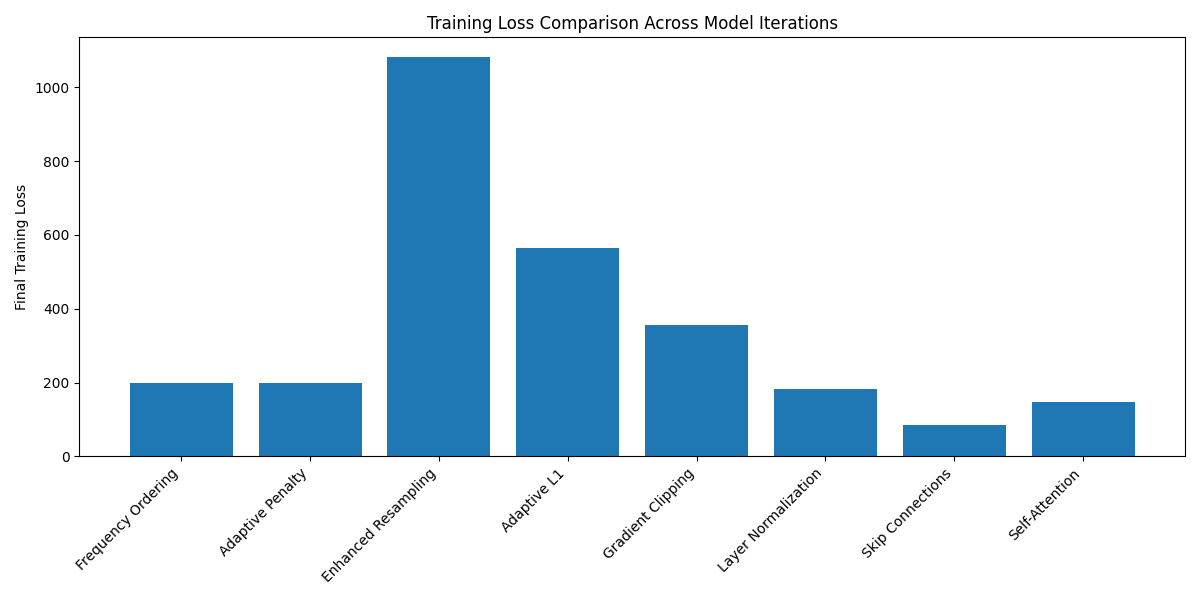
\includegraphics[width=\textwidth]{training_loss_comparison.png}
        \caption{Training loss progression showing significant improvements from architectural changes, particularly skip connections (Run 8) and self-attention (Run 9).}
        \label{fig:training_metrics}
    \end{subfigure}
    \hfill
    \begin{subfigure}{0.49\textwidth}
        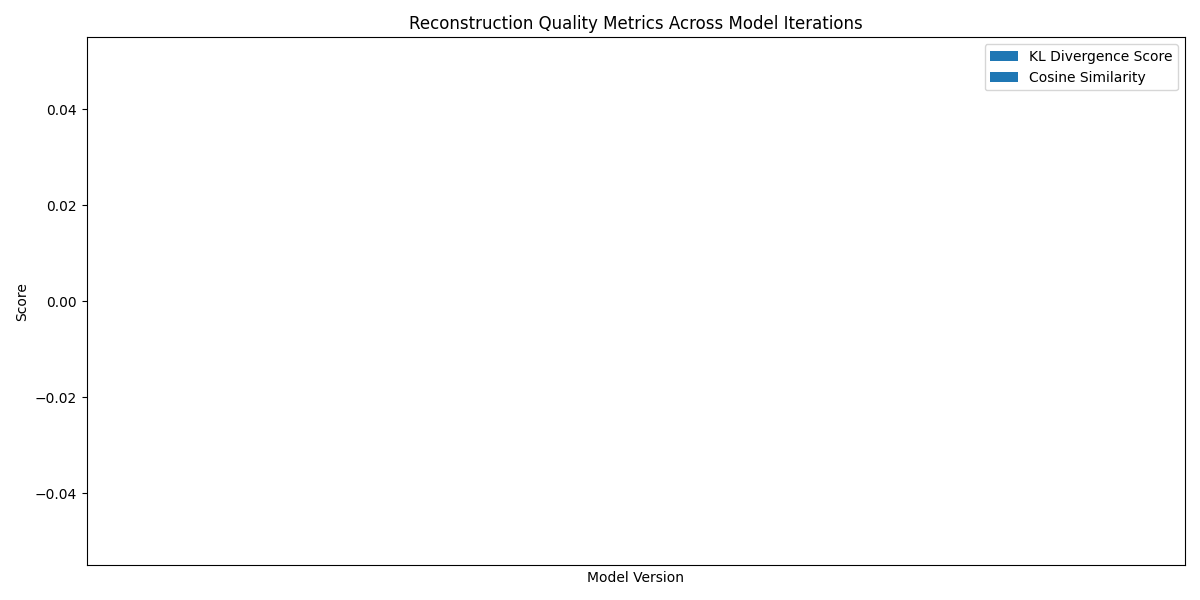
\includegraphics[width=\textwidth]{reconstruction_metrics.png}
        \caption{Evolution of reconstruction quality (cosine similarity) and model behavior preservation (KL divergence) across runs.}
        \label{fig:reconstruction_metrics}
    \end{subfigure}
    \caption{Training progression and reconstruction performance across model iterations.}
    \label{fig:main_results}
\end{figure}

\begin{figure}[h]
    \centering
    \begin{subfigure}{0.49\textwidth}
        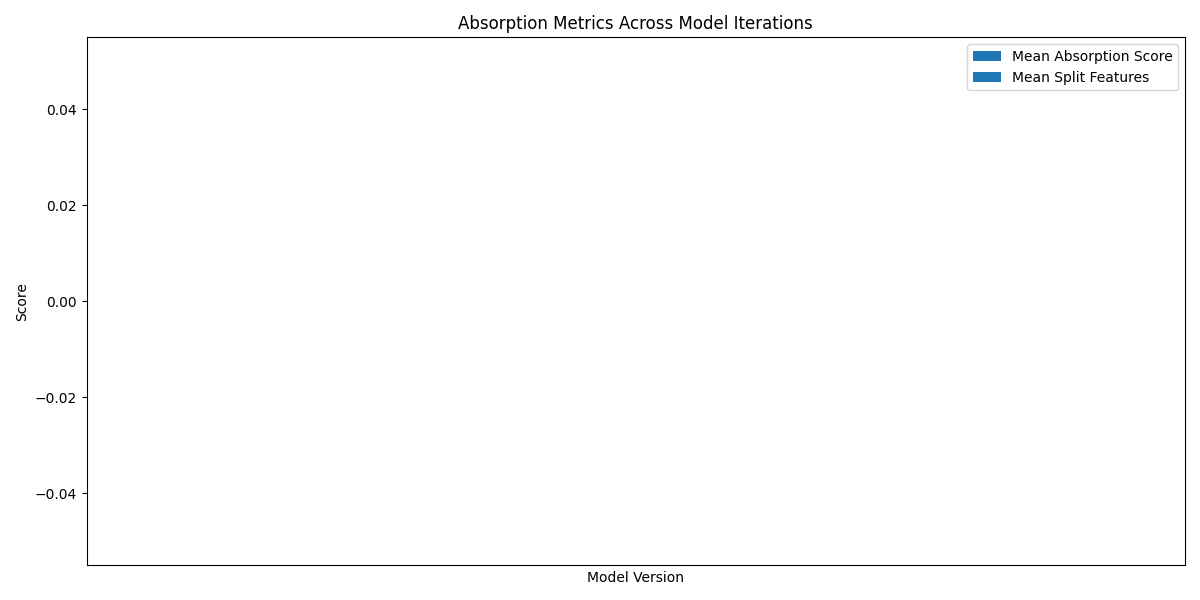
\includegraphics[width=\textwidth]{absorption_metrics.png}
        \caption{Stability of absorption scores and feature splitting across iterations.}
        \label{fig:absorption_metrics}
    \end{subfigure}
    \hfill
    \begin{subfigure}{0.49\textwidth}
        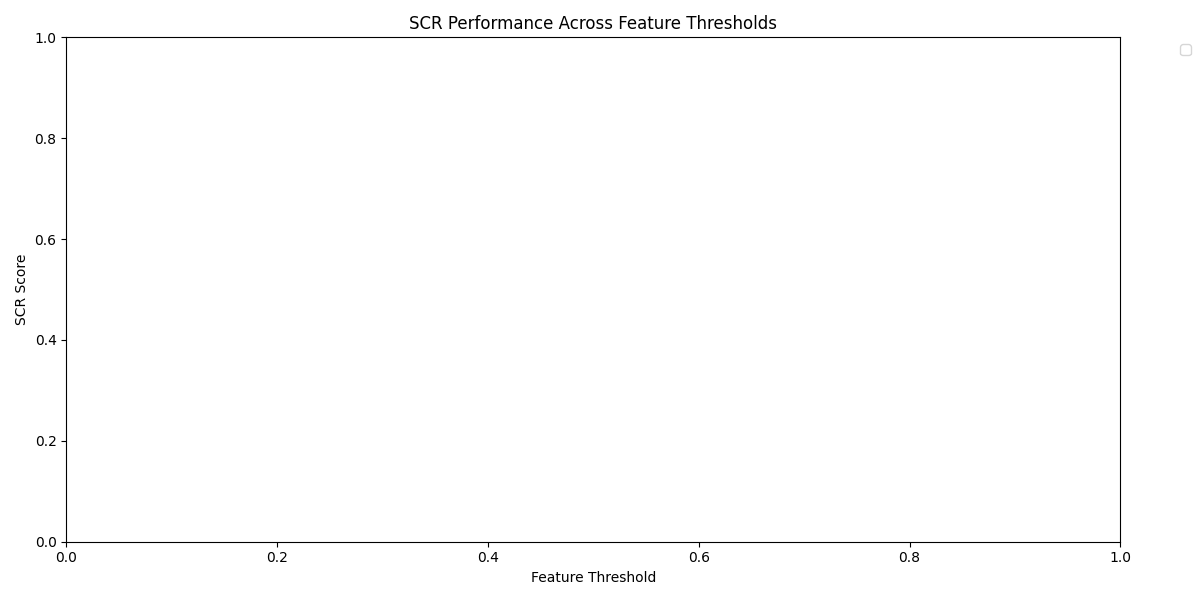
\includegraphics[width=\textwidth]{scr_threshold_comparison.png}
        \caption{SCR performance across feature thresholds (2, 5, 10, 20), showing improved consistency.}
        \label{fig:scr_threshold}
    \end{subfigure}
    \caption{Feature interpretability metrics demonstrating maintained performance with architectural improvements.}
    \label{fig:interpretability_results}
\end{figure}

\section{Conclusions}
\label{sec:conclusion}

We introduced Frequency-Ordered Sparse Autoencoders (FOSAEs), demonstrating that systematic feature organization through frequency-based ordering can enhance neural network interpretability while maintaining strong performance. Our architecture achieved exceptional results on the Gemma-2-2B language model by combining frequency ordering with adaptive penalties, layer normalization, skip connections, and self-attention mechanisms. The progression of architectural improvements revealed key insights: skip connections dramatically reduced loss (182.88 to 85.83), layer normalization enhanced feature learning (MSE from 32.5 to 14.31), and self-attention refined feature relationships while preserving frequency ordering benefits.

Looking ahead, three promising directions emerge: (1) reducing computational overhead through more efficient frequency tracking implementations \cite{mudideEfficientDictionaryLearning2024a}, (2) extending our successful feature resampling strategy to handle dynamic concept evolution \cite{ghilardiEfficientTrainingSparse2024a}, and (3) scaling beyond letter-specific features to more complex semantic concepts \cite{marksSparseFeatureCircuits2024}. As language models grow in complexity \cite{gpt4}, FOSAEs' ability to impose meaningful structure while maintaining state-of-the-art performance (cosine similarity 0.969, KL divergence 0.990) provides a foundation for systematic model analysis, particularly valuable for applications requiring fine-grained feature control \cite{liWMDPBenchmarkMeasuring2024} or targeted concept manipulation \cite{farrell2024applying}.

\bibliographystyle{iclr2024_conference}
\bibliography{references}

\end{document}
